\part{Entwicklerhandbuch}

\chapter{Übersicht}
\section{Technologien und Werkzeuge}
Um die Anforderungen an das Software-Projekt bestmöglich zu erfüllen werden verschiedene Web-Technologien und -Werkzeuge zur Umsetzung des Projektes verwendet. Im folgenden wird erläutert, an welcher Stelle des Projektes diese eingesetzt werden und warum.

\paragraph{Javascript}Die Skriptsprache \textit{Javascript} wird im vorliegenden Projekt als Programmiersprache verwendet. Der aktuelle \textbf{ECMA-262}\footnote{\url{http://www.ecma-international.org/publications/standards/Ecma-262.htm}} Standard ermöglichte dabei eine objektorientierte Implementierung unter anderem mit der Verwendung von Klassen.

\paragraph{node.js}Um die Ausführung von Javascript-Code außerhalb eines Browsers zu ermöglichen wird die Laufzeitumgebung \textit{node.js} verwendet.

\paragraph{React.js}Durch die Nutzung des Javascript-Frameworks \textit{React.js} ist es möglich die Benutzerschnittstelle besonders effizient zu rendern. Dafür wird unter anderem ein spezieller \textit{React-Syntax} gewählt, welcher mit sogenannten \textit{React-Objekten} arbeitet. Das Framework verwendet diese um beim rendern eines Folgeframes ausschließlich jene Bereich zu erneuern, welche sich tatsächlich verändert haben.

\paragraph{npm}Um die Erfüllung von Abhängigkeiten im Laufe der Implementierung elegant und automatisiert zu gewährleisten wird die Javascript-Paketverwaltung \textit{npm} genutzt. Diese wird über die Datei \texttt{package.json} im Root-Verzeichnis der Anwendung konfiguriert.

\paragraph{bower}Während \textit{npm} vorrangig Backend-relevante Pakete verwaltet, ist die Paketverwaltung \textit{bower} auf Frontend-spezifische spezialisiert. So wird bower beispielsweise verwendet um Pakete wie \textit{bootstrap} oder \textit{React.js} einzubinden. Die Konfiguration findet hier ähnlich zu \textit{npm} über eine Kon"-fi"-gu"-ra"-tionsdatei (\texttt{bower.json}) statt.

\paragraph{grunt}Bei der Implementierung der Anwendungen wird Javascript nach \textit{ES6-Standard} und \textit{LESS} zur Beschreibung der Styles benutzt. Selbst moderne Browser unterstützen dieses Technologien jedoch noch nicht umfassend, weshalb verschiedene Transpiler notwendig sind. Diese und weitere Aufgaben werden mit Hilfe des \textit{grunt}-Framworks verwaltet und automatisiert durchgeführt. Die Datei \texttt{Gruntfile.js} enthält die Konfiguration des Tools.

\paragraph{karma \& jasmine}Neben manuellen Software-Tests wurden im Rahmen des Projektes ebenfalls automatisierte Testverfahren entworfen und angewendet. Die Kombination der Tools \textit{karma} und \textit{jasmine} bilden dazu das verwendete Framework.


\section{Systemvoraussetzungen}
Neben einem beliebigem Texteditor benötigt man zur Weiterentwicklung der Anwendung zunächst das \textit{node.js}-Framework. Dieses kann unter folgender url:\url{https://nodejs.org} für verschiedene Plattformen bezogen werden.

\paragraph{}Nach der Installation von \textit{node.js} können alle weiteren Pakete und Werkzeuge mit Hilfe der Paketverwaltung \textit{npm} nachgeladen werden. Diese ist Teil der \textit{node.js}-Installation. Um diese zu tun sind folgende Befehle mit Administratorrechten in einer Kommandozeile einzugeben:

\begin{lstlisting}
	npm install -g nw
	npm install -g grunt
	npm install -g bower
	npm install
	bower install
\end{lstlisting}

Nach der Installation dieser Pakete sind alle Systemvoraussetzungen für Weiterentwicklung dieser Anwendung erfüllt. 

\section{Build-Prozess}
Wie bereits mehrfach erwähnt war die große Kompatibilität zu verschiedenen Plattformen ein Grund für die Entscheidung, das Projekt mit Web-Tech”-no”-lo”-gien umzusetzen. Als \textit{Build-Prozess} wird in diesem Kontext die Routine bezeichnet, die aus dem Quellcode des Projektes die Pakete erzeugt, welche an Kunden und Benutzer ausgeliefert werden.

\paragraph{}Der \textit{Build-Prozess} wurde im vorliegenden Projekt mit Hilfe des \textit{grunt}-Frame"-works automatisiert und soll im folgenden beschrieben werden. Diese Beschreibung eignet sich zusätzlich als Einführung in die Arbeitsweise des \glqq Task-Runners \grqq \textit{grunt}. Dargestellte Listings sind der \textit{grunt}-Kon"-fi"-gurations"-datei \\\texttt{Gruntfile.js} entnommen.

\begin{lstlisting}[language=JavaScript,label=JS:grunt_build,caption=grunt build-Task]
grunt.registerTask('build', function (target) {
	grunt.task.run([
		'dist',
		'nodewebkit',
	]);
});
\end{lstlisting}

Zeile 1 im Listing \ref{JS:grunt_build} zeigt die \glqq Anmeldung\grqq des Tasks im Framework. Dies hat zur Folge das der beschriebene Task im Wurzelverzeichnis der Anwendung durch Eingabe des folgenden Befehls in einer Kommandozeile \texttt{grunt serve} ausgeführt werden kann. Dieser Task bündelt nun die Ausführung von \texttt{dist} und \texttt{nodewebkit}.

\newpage
\begin{lstlisting}[language=JavaScript,label=JS:grunt_dist,caption=grunt dist-Task]
grunt.registerTask('dist', function (target) {
	grunt.task.run([
		'clean:dist',
		'useminPrepare',
		'concurrent:dist',
		'postcss',
		'concat',
		'cssmin',
		'uglify',
		'copy:dist',
		'filerev',
		'usemin',
		'htmlmin',
	]);
});
\end{lstlisting}

\paragraph{}Listing \ref{JS:grunt_dist} zeigt den Inhalt des \textit{dist}-Tasks. Die einzelnen Punkte entsprechen wiederum verschiedenen Unteraufgaben, welche in Tabelle \ref{dist_table} näher beschrieben sind.

\paragraph{}Diese Aufgaben dienen alle der Vorbereitung des Quellcodes um im Anschluss mittels \texttt{nodewebkit} die fertigen Anwendungen zu erstellen. Listing \ref{JS:grunt_webkit_config} zeigt die Konfiguration der entsprechenden Aufgaben. Neben Quell- und Zielordner sind hier die jeweiligen Zielarchitekturen eingetragen.

\begin{tabularx}{0.92\textwidth}{lX}
	\textit{clean:dist} & bereinigt temporäre und build-Ordner\\ \hline
	\textit{useminPrepare} & TODO\\ \hline
	\textit{concurrent:dist} & Konfiguriert verschiedene Unteraufgaben um Nebenläufigkeit im Build-Prozess zu erzeugen\\ \hline
	\textit{postcss} & TODO\\ \hline
	\textit{concat} & TODO\\ \hline
	\textit{cssmin} & Verringert die Größe der CSS-Dateien\\ \hline
	\textit{uglify} & Verringert die Größe der Javascript-Dateien\\ \hline
	\textit{copy:dist} & Kopiert alle notwendigen Dateien in die jeweiligen Veröffentlichungs-Unterordner\\ \hline
	\textit{filerev} & Ändert Dateinamen um Probleme mit dem Cache des Browser zu vermeiden\\ \hline
	\textit{usemin} &  TODO\\ \hline
	\textit{htmlmin} & Verringert die Größe der HTML-Dateien\\ \hline
\end{tabularx}
\label{dist_table}
\vspace*{1cm}

\begin{lstlisting}[language=JavaScript,label=JS:grunt_webkit_config,caption=grunt nodewebkit-Konfiguration]
nodewebkit: {
	options: {
		platforms: [
			'win32',
			'win64',
			'linux32',
			'linux64',
			'osx64',
		],
		buildDir: 'builds',
	},
	src: ['dist/**/*'],
},
\end{lstlisting}

\paragraph{}Nach Abschluss dieses Tasks befinden sich die Versionen zur Veröffentlichung in Unterordnern \texttt{ win32, win64, linux32, linux64} und\texttt{ osx64 }des Ordners \texttt{ dist } im Wurzelverzeichnis der Anwendung.

\chapter{Software-Entwurf}
\section{Grobentwurf}
Eine Prämisse des Projektes war stets den Fahrstuhl inklusive Steuerung mög"-lichst realitätsnah zu simulieren. Daher wurde die Anwendung von Beginn an in Teilsysteme untergliedert.

\paragraph{Komponentenstrukt}Dies zeichnet sich insbesondere in der Struktur der Anwendung aus, welche aus mehrere Komponenten besteht, die wiederum in der Realität existierende Teilsysteme eines Fahrstuhlsystems abbilden. So unterteilt sich das Gesamtsystem \textbf{Fahrstuhlsimulation} zunächst in die Teilsysteme \textbf{Fahrstuhlsteuerung} und \textbf{Visualisierung}, welche weiterhin verschiedene Komponenten beinhalten.

\paragraph{}Im Entwurf der \textbf{Fahrstuhlsteuerung} sind dementsprechend \textit{Steuerung}, \textit{Sensoren} und \textit{Schnittstellen zur Passagierinteraktion} in voneinander unabhängige Komponenten gekapselt, welche sich im Feinentwurf auch als Klassen des Software-Systems wiederfinden.

\paragraph{}Zu den Sensoren der Fahrstuhlsimulation gehören \textit{Etagen-}, \textit{Tür-}, und \textit{Gewichtssensoren}. Deren Kommunikation mit der Steuerung erfolgt ebenfalls über definierte Schnittstellen, wobei zusätzlich zu unterscheiden ist, ob es sich um aktive oder Passive Sensoren handelt.\todo{Welche Sensoren sind aktiv, welche Passiv?}

\paragraph{MVC-Paradigma}Auf einer hohen Abstraktionsebene kann das System so auch unter dem MVC-Modell\footnote{Abk. für Model-View-Controler-Modell } betrachtet werden. Die Intention besteht darin die Fahrstuhlsteuerung als Modell zu charakterisieren und die Kommunikation mit der Benutzerschnittstelle, der View, über einen Controller zu etablieren. Somit Kommunizieren die verschiedenen Teilsysteme ausschließlich über definierte Schnittstellen und die Paradigmen Modularität und Wiederverwendbarkeit sind inhärent erfüllt.

\paragraph{Steuerungs-Algorithmus}Neben der Struktur der Anwendung ist ebenfalls ein aus der Realität bekannter Algorithmus zur Steuerung des Fahrstuhls adaptiert worden, der sogenannte \textit{Fahrstuhl-Algorithmus mit Sammelsteuerung}\cite{wiki_elev}. Dieser bedient zunächst Fahrtwünsche und -Rufe auf der aktuellen Fahrtrichtung und kehrt diese im Anschluss um.

\paragraph{}Die Fahrstuhlsteuerung muss nun beim Erreichen einer Etage unter anderem zwei Fragen beantworten:

\begin{enumerate}
	\item Existiert ein Fahrtwunsch /-Ruf auf dieser Etage und muss dementsprechend angehalten werden?
	\item Existieren Fahrtwünsche /-Rufe ober- oder unterhalb der aktuellen Etage, beziehungsweise muss die Fahrtrichtung beibehalten oder umgekehrt werden?
\end{enumerate}

\paragraph{}Frage 2. ist in dem Fall die interessantere. Ein naiver Ansatz könnte folgendermaßen außen:\\ \\ Ein System besitzt $N$ Etagen, die Kabine befindet sich aktuell in Etage $M$ und fährt in Richtung $X$. Um zu entscheiden ob die Fahrt in der aktuellen Fahrtrichtung fortgesetzt wird durchsucht die Steuerung die Datenstruktur der Etagen linear im Bereich $(M,N]$ für $X>0$ (aufwärts) oder im Bereich $[0,M)$ für $X<0$ (abwärts).\\\\
Dieser Algorithmus wäre jedoch abhängig von der Menge der Etagen und besäße damit die Komplexität $\mathcal{O}(n)$.

\paragraph{}Beim Entwurf des Algorithmus der vorliegenden Anwendung war das Ziel diese Komplexität zu verringern. Seine Funktion erklärt sich wie folgt:\\ \\ Grundlegendes Element des Algorithmus ist eine Datenstruktur, welche ausschließlich die \textbf{Summe} der Fahrtwünsche /-Rufe über- und unterhalb der aktuellen Position enthält. Um nun über die Fahrtrichtung entscheiden zu können muss die Fahrstuhlsteuerung ausschließlich an definierten Stellen in dieser Datenstruktur überprüfen, ob Elemente größer 0 sind. Die Komplexität dieser Abfrage über einer Datenstruktur fester Größe besitzt die Komplexität $\mathcal{O}(1)$, was einer Reduktion entspricht. Zu beachten ist dabei jedoch, dass die genannte Datenstruktur zu jedem Zeitpunkt aktuell gehalten werden muss. Dies ist jedoch ein implementierungsspezifisches Problem, dessen Lösung in der Sektion \textit{\nameref{onLevelContact}} im Kapitel \textbf{\nameref{imp}} beschrieben wird.

\section{Feinentwurf}

\paragraph{MVC - React \& FLUX}
\todo{hier muss erklärt werden wie ReactJS funktioniert und warum es die Performance verbessert}
\paragraph{Observer Pattern}
\paragraph{Klassendiagramm}
\begin{figure}[h!]
	\centering
	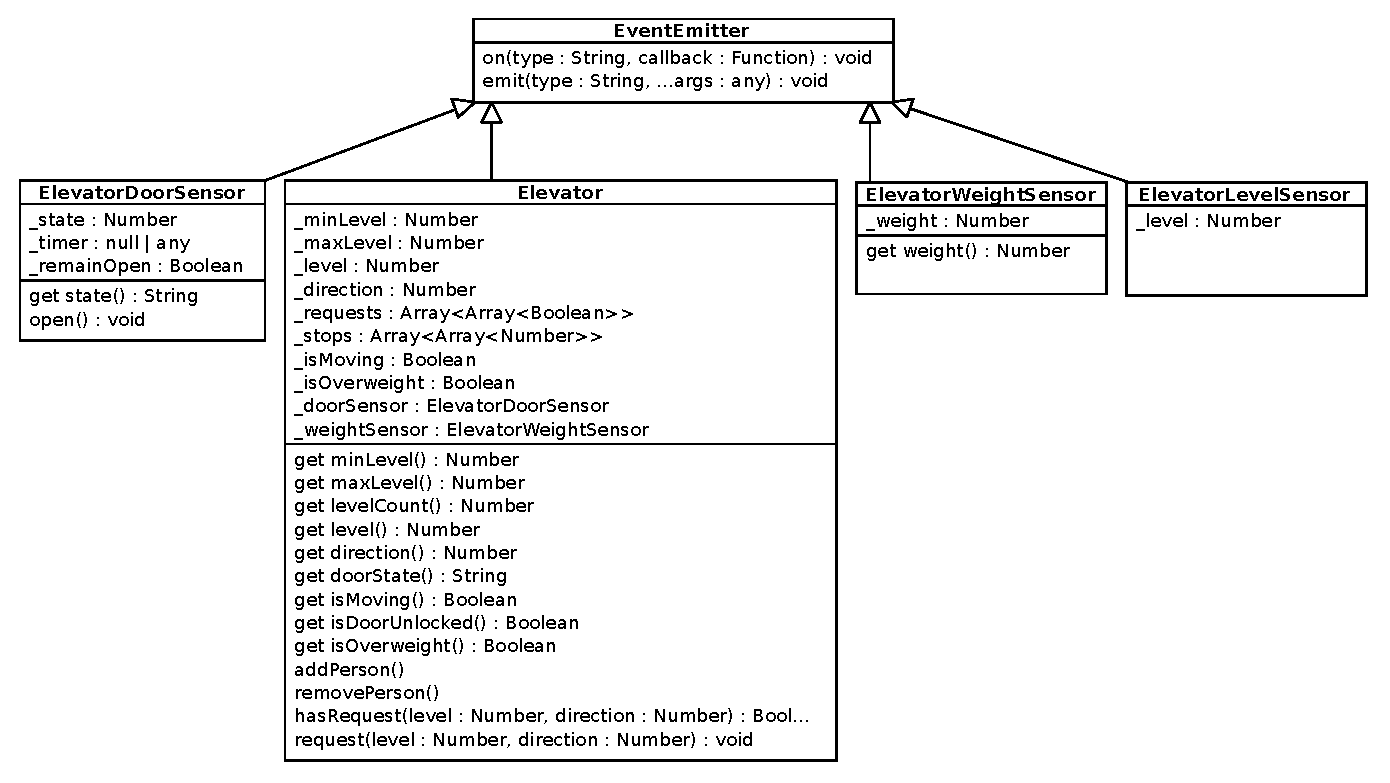
\includegraphics[width=0.9\textwidth]{images/klassendiagramm.eps}
	\caption{Übersicht der verwendeten Klassen der Hauptkomponente Fahrstuhlsteuerung}
	\label{klassdiagramm}
\end{figure}
\chapter{Implementierung}
\label{imp}

\section{Elevator emitMove Levelsensor onLevelContact}
\label{onLevelContact}

\section{Benutzerschnittstelle}
Damit die aktiven Zustände hervorgehoben werden können, müssen sie eindeutig identifizierbar sein. Dafür wurden die Elemente der Grafik gruppiert und mit IDs versehen, auf die mittels Javascript und dem \acrshort{DOM} zugegriffen werden kann. Abbildung \ref{fig:ZD_id_view} stellt die Identifikatoren dar. Bei der Benennung der IDs wurden folgende Konventionen angwendet:
\begin{itemize}
	\item präfix uml- für alle Bezeichner
	\item Worte durch Bindestriche getrennt
\end{itemize}

\begin{figure}[hbt]
	\centering
	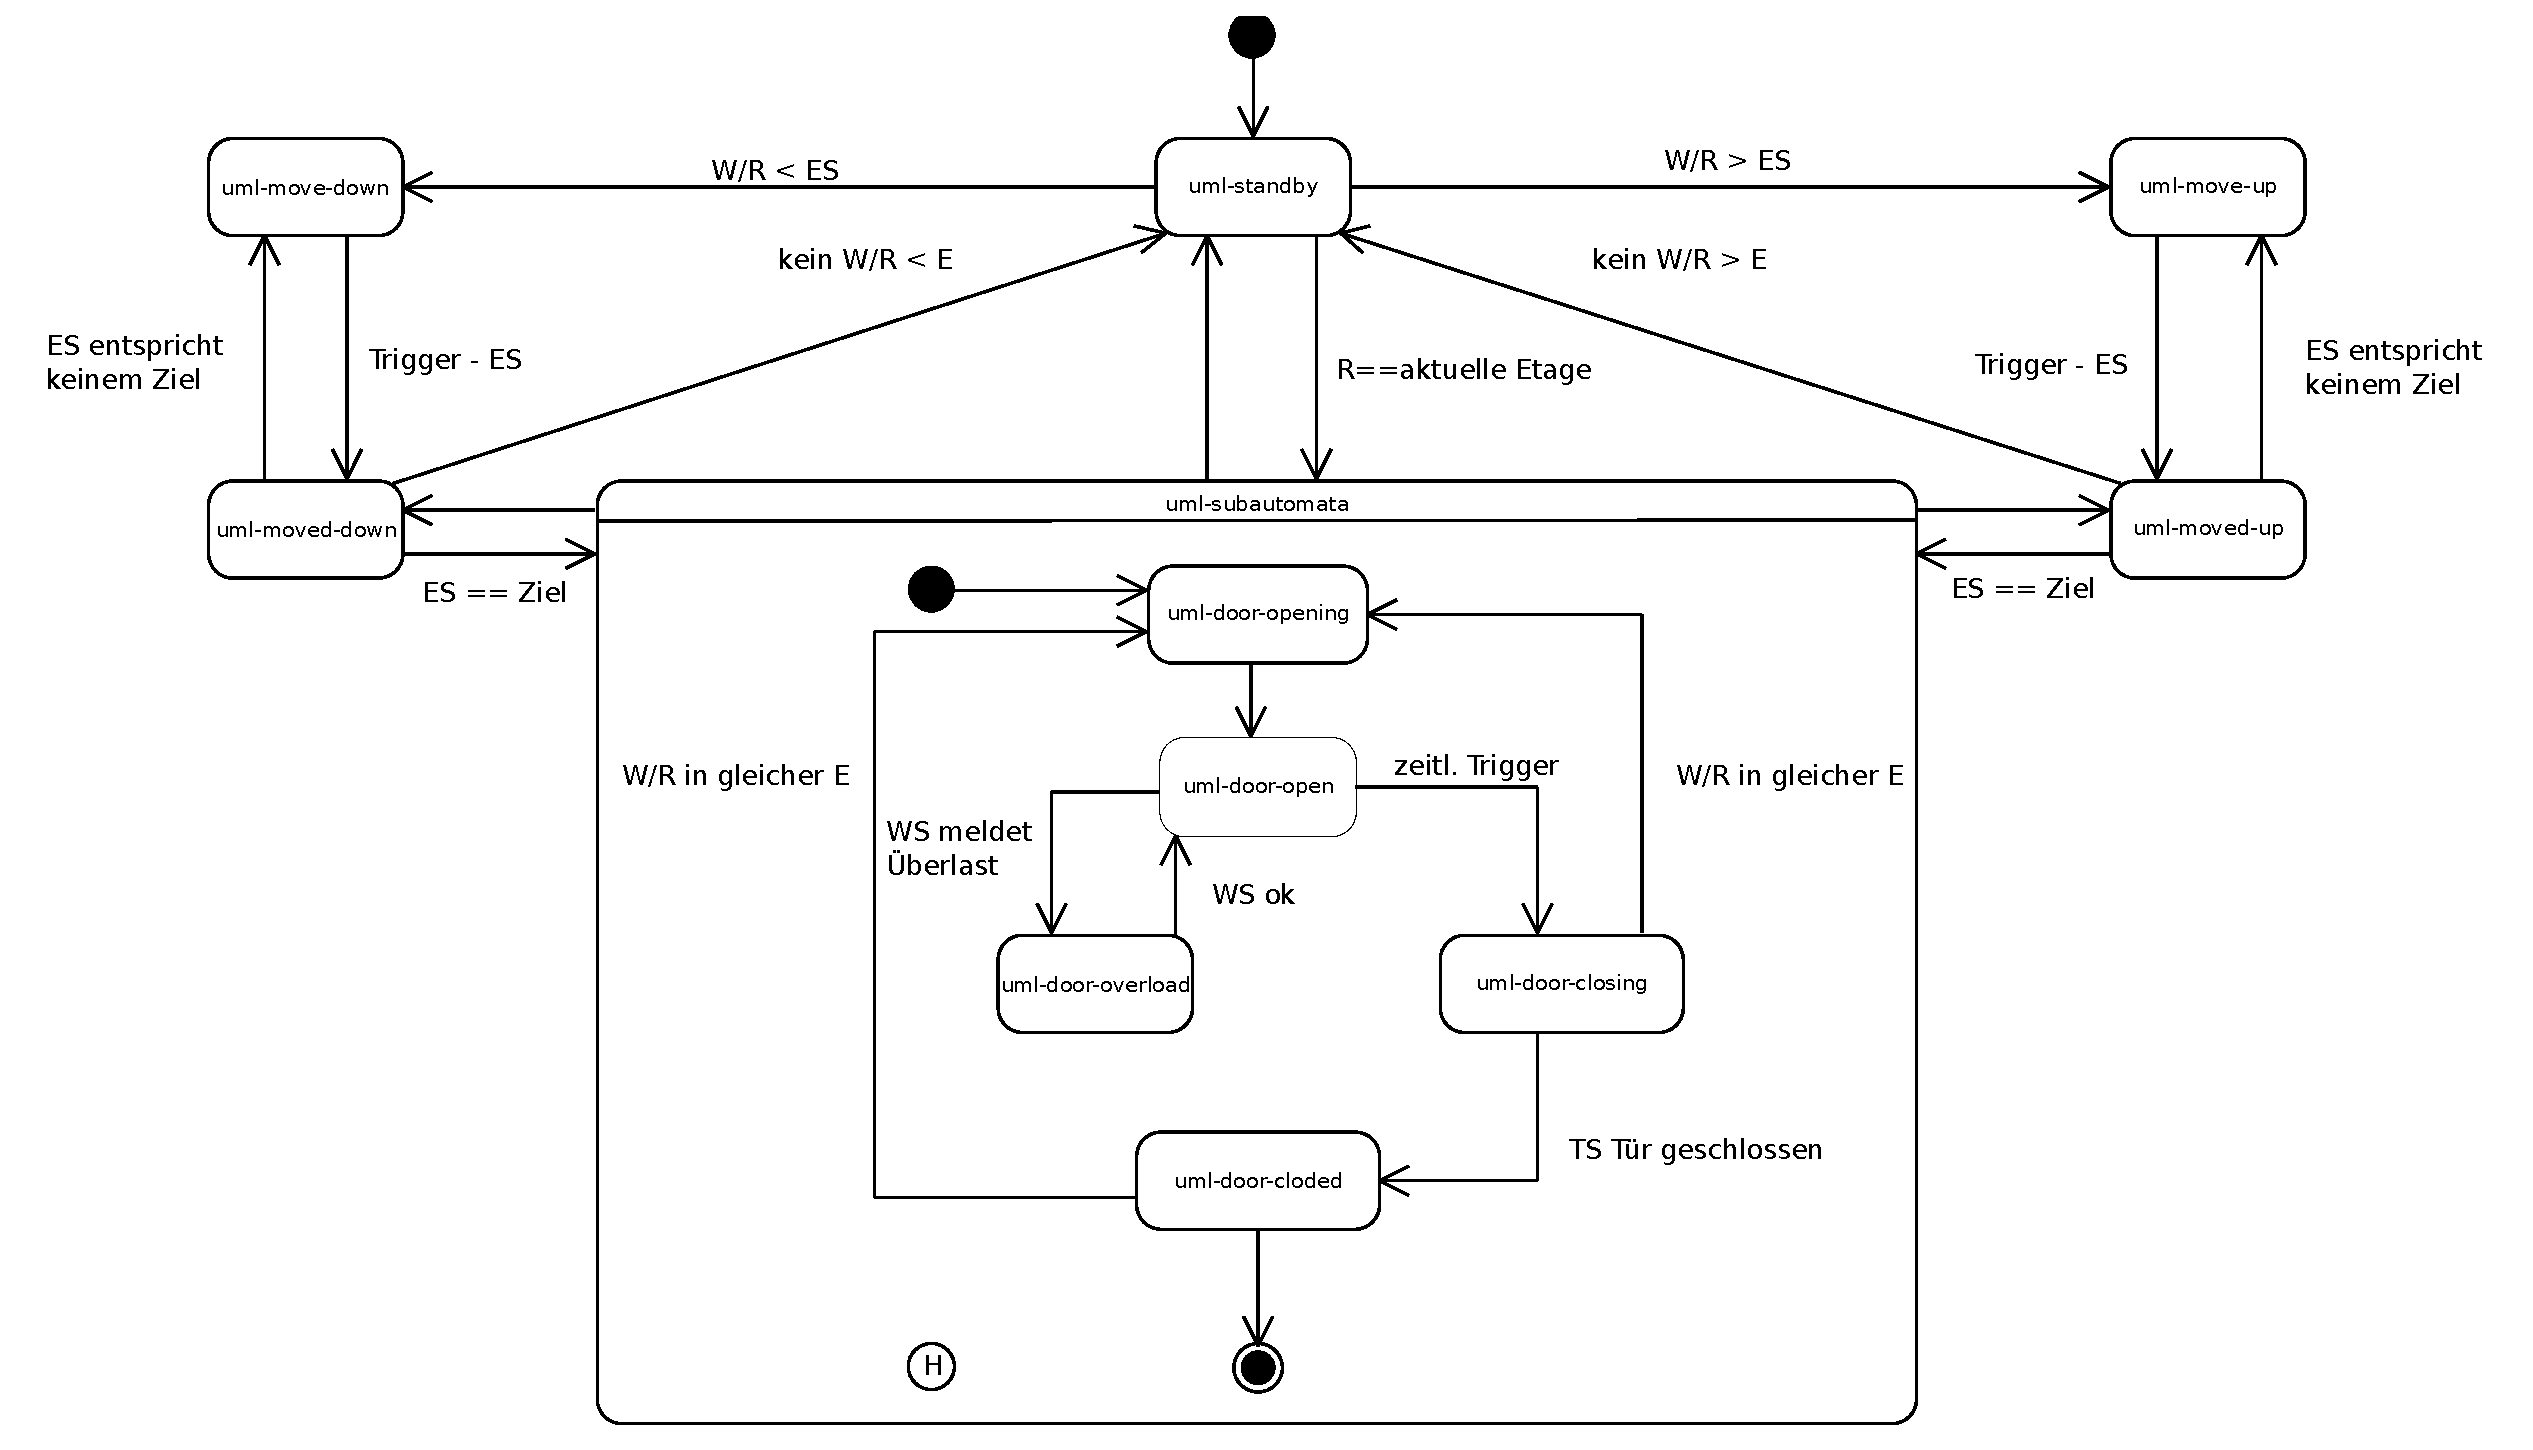
\includegraphics[width=\textwidth]{images/ZDv6_id_view.eps}
	\caption{IDs des Zustandsdiagrammes}%
	\label{fig:ZD_id_view}%
\end{figure}

\section{API}

\section{Erweiterungen}

